\subsect{Sprint 1}{sprint1}

\underline{Fecha de inicio}: 11/06/2022

\underline{Fecha de fin}: 11/07/2022

\underline{Objetivo}:
Crear un prototipo de la aplicación.

\underline{Descripción}:
En este sprint se pretende crear un prototipo de la aplicación, con el fin de tener una primera versión
que se pueda probar y que sirva como base para el desarrollo de la versión final.\ Se desarrollará
una API con seguridad básica y se creará una aplicación web que consuma dicha API\@.\ Las rutas de la última\@,
se dividirán según el tipo de petición que se realice, es decir, habrá rutas para las peticiones GET, POST, PUT y
DELETE\@.\ Se creará una base de datos con los modelos necesarios para la aplicación y se crearán los controladores
para que la API funcione correctamente.\ Se creará una aplicación web con React que la consuma y que
permita realizar las operaciones básicas de la aplicación.\ Además, es necesario un endpoint que permita
la conexión por WebSocket al servidor, para poder realizar la comunicación en tiempo real entre los usuarios.

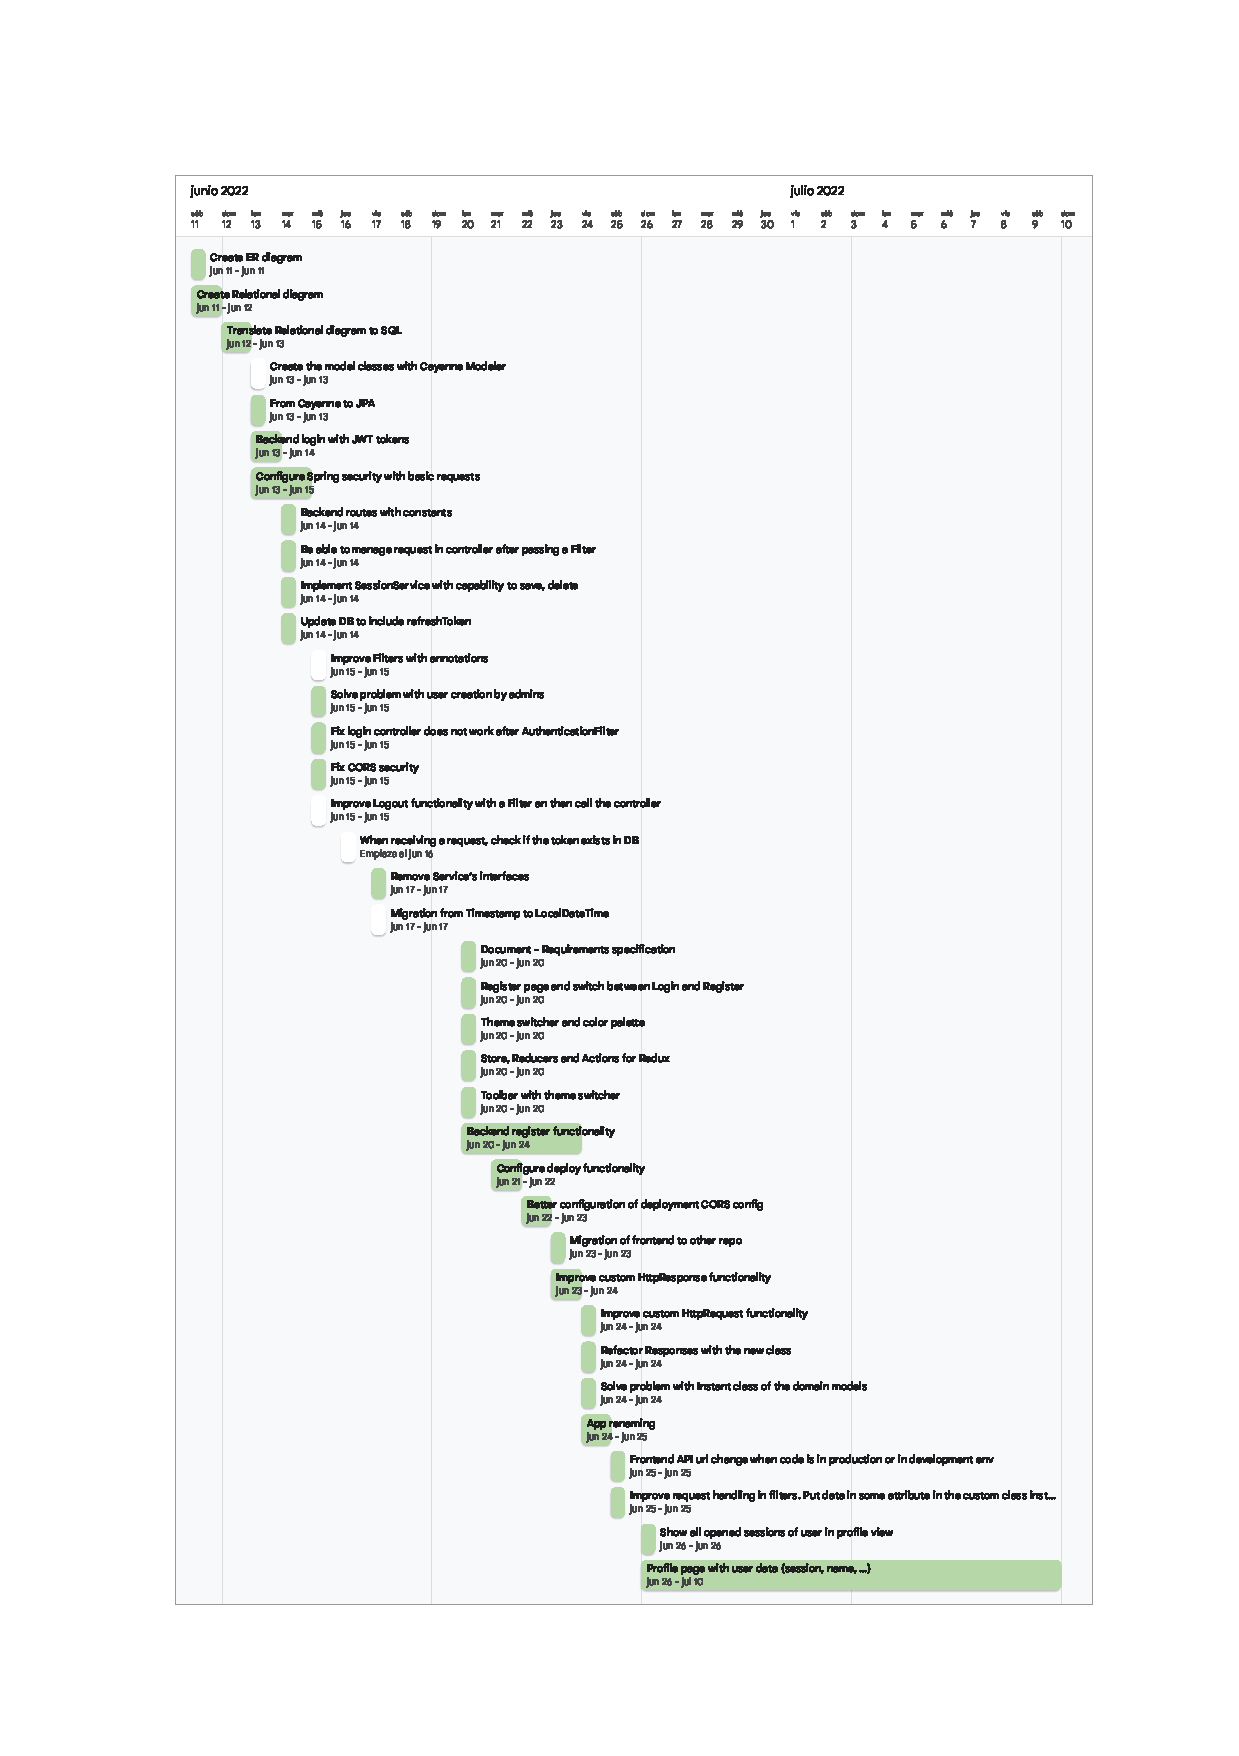
\includepdf[pages=-]{backlog/sprints/Sprint1.pdf}
